%Objectives : 
%\begin{itemize}
%    \item Present the rising velocity Vs. phi to demonstrate the relation with $\phi^{1/3}$ \citep{loisy2017buoyancy}
%    \item Discus the common points and differences with bubbles and solid particles. 
%    \item Present a proper definition of the drag force terms such as in \citet{wang2021numerical}. 
%    \item Discus the possible correlation between the shape /arrangement of the particles/flow lines with the rising velocity. \tb{Je ne sais pas trop quoi dire la dessus}
%    \item Show that \citet{rusche2000effect}'s fit for the drag force is not adapted for our case and propose a new one
%    \item All the references for teh Drag force terms are in \citet[chap 8]{morel2015mathematical} or in \citet{ishii2010thermo}
%\end{itemize}
%\todo[inline]{include fits of bubbly flow}


%\JL{bien expliquer que ce que l'on mesure c'est les vitesses donc si on veut faire un modèle il faut repartir des vitesses (leur difference plus specifiquement). la pseudo turbulence entre elle dans la pression ou dans la viscosité ?}



%\begin{equation}
% F = ...
%\end{equation}
%On peut aussi parler du gradient de pression.


%The main difficulty is to relate the force to the flow parameters relative velocity between the two phases. 


In this section, we start by reviewing the various existing models for the averaged drag force acting on fluid inclusions in the Stokes regime. Subsequently, we consider the intermediate Reynolds number regime, the primary focus of our current investigation, proposing a drag model that reasonably fits the numerical results. As demonstrated in \ref{app:shape}, the droplet maintains an approximate spherical shape within the range of parameters studied here. Although slight deviations from sphericity are noted for $Bo=1$ and in configurations with the highest inertia, the maximum deviation from the spherical shape remains moderate less than $12$ \%. Hence, in this section we assume that fluid inclusions are spherical.

%. Henceforth, for the entirety of this section, we adopt the assumption that fluid inclusions exhibit spherical characteristics.

%Then we consider the intermediate Reynolds number regime studies which is the focus of the present work and propose a drag model which reasonably fits the numerical results. As demonstrated in Appendix \ref{app:shape} the droplet remains approximatively spherical within the range of parameters studied presently. Although some deviation from sphericity are observed for $Bo=1$ and in the highest inertial configurations the maximum deviation from the spherical shape remains moderate at around $10$ \%. Thus within the whole section, we will assume that the fluid inclusions are spherical. 


%In this section, we commence by examining existing models that describe the averaged drag force acting on fluid inclusions in the Stokes regime. Subsequently, we delve into the intermediate Reynolds number regime, the primary focus of our current investigation, proposing a drag model that effectively aligns with numerical results. As elucidated in Appendix \ref{app:shape}, the droplet maintains an approximate spherical shape within the studied parameter range. Although slight deviations from sphericity are noted for $Bo=1$ and in configurations with the highest inertia, the maximum departure from spherical shape remains modest at approximately 10%. Henceforth, for the entirety of this section, we adopt the assumption that fluid inclusions exhibit spherical characteristics.
  
%This assumption remains valid for the whole range of parameters investigated

\subsection{ The momentum balance in homogeneous sedimentation}

\paragraph{Relation between forces and buoyancy :} The momentum conservation equations in the restricted situation of homogeneous sedimentation of particles reads from \ref{eq:dt_uc} and \ref{eq:dy_up} :
\begin{align}
    % \pddt (\phi_f\rho_f \textbf{u}_f)
    % + \div \left(\phi_f\rho_f \textbf{u}_f\textbf{u}_f + \phi_f  \bm{\sigma}_f^{\text{Re}} - n_p\textbf{M}_p \right)
    0 
    &= \phi_f 
    \left(\div \bm{\sigma}_f
    + \rho_f \textbf{g}\right)
    - n_p \textbf{f}_p, 
    \label{eq:dt_uf_steady}
    \\
    % \pddt (\phi_d\rho_d \textbf{u}_p)
    % + \div \left(\phi_d\rho_d \textbf{u}_p\textbf{u}_p+ \phi_d \bm{\sigma}_p^{\text{Re}}\right)
    0
    &= 
    \phi_d \left(\div \bm{\sigma}_f
    + \rho_d \textbf{g}\right)
    + n_p \textbf{f}_p. 
    % \label{eq:dy_up}
    \label{eq:dt_up_steady}
\end{align}
multiplying \ref{eq:dt_uf_steady} by $\phi_d$ and \ref{eq:dt_up_steady} by $\phi_f$ and subtracting the resulting equations gives, 
\begin{align}
    n_p \textbf{f}_p
    &= 
    \phi_d \phi_f (\rho_f -\rho_d ) \textbf{g}
    % \label{eq:dy_up}
\end{align}
In  mono-disperse suspension of droplets $n_p = \phi_d / v_p$ with $v_p =4/3\pi d^3/8$ the volume of a particle which yields the final results, 
\begin{equation*}
    \textbf{f}_p
    = 
    \frac{4}{3}\pi\frac{d^3}{8}\phi_f (\rho_f -\rho_d ) \textbf{g}
    \label{eq:drag}
\end{equation*}
It is convinient to make dimensionless this force with Hadamard-Ribczynski formula, which is, 
\begin{equation*}
    \textbf{f}^0_p = \pi \mu_f d A \textbf{u}_{pf}
\end{equation*}
Dividing one by the other gives the dimensionless force
\begin{equation*}
    \textbf{f}^*_p 
    = 
    \frac{4}{3A}\frac{d^2 \phi_f (\rho_f -\rho_d ) \textbf{g}}{8 u_{pf}\mu_f}
\end{equation*}
This can be made dimensionless with $\phi_f$



\paragraph{Relation between buoyancy and drag coefficient :}
We assume that the force can be written in the form, 
\begin{equation*}
    \textbf{f}_p = C_d  \pi \rho_f \frac{d^2}{8} u_{pf}^2
\end{equation*}
where $C_d$ is a dimensionless coefficient and $\textbf{u}_{fp}$ is the relative phase velocity. 
Using \ref{eq:drag} we show that $C_d$ coefficient is related to the relative velocity with, 
\begin{equation*}
    C_d  
    = 
    \frac{4}{3}
    \frac{d \phi_f (\rho_f -\rho_d ) \textbf{g}}{\rho_f u_{pf}^2}
\end{equation*}
This can be directly computed into our DNS. 
\begin{equation*}
    C_d  \phi_f^2 \frac{\rho_f^2 d^2 u_{pf}^2}{\mu_f^2}
    = 
    \frac{4}{3}
    \phi_f^3 
    \frac{
        d^3
        \rho_f
        (\rho_f -\rho_d ) g
    }{\mu_f^2}
\end{equation*}
Let us define the Galileo number as $Ga^2 = \frac{
    d^3
    \rho_f
    (\rho_f -\rho_d ) g
}{\mu_f^2}$ and the Reynolds number based on the drift velocity as, $Re =  \phi_f \frac{\rho_f d u_{pf}}{\mu_f}$,
Then, the relation between the Reynolds and Galileo is given by, 
\begin{equation*}
    Re
    = 
    Ga
    \sqrt{\frac{4\phi_f^3}{3 C_d}}
\end{equation*}
This the relative velocity is given by, 



In stokes and dilute regime the $C_d$ noted $D_c^0$ is given by Hadamard-Ribczynski solution and reads, 
\begin{equation*}
    C_d^0 = \frac{8}{Re} \left(\frac{3\lambda +2 }{\lambda +1}\right)
    = \frac{8}{Re}A
\end{equation*}
where we introduced the constant $A = \left(\frac{3\lambda +2 }{\lambda +1}\right)$. 
Thus, the Reynolds number obtained for a given \textit{Galileo} number in stokes regime is, 
\begin{equation*}
    Re^0
    = 
    \frac{Ga^2}{6 A}
    % \phi_f^3  
\end{equation*}
Since this is valid for an isolated particle we fixed $\phi_f=1$, this will be our renormalization constant. 
\begin{equation*}
    Re^*
    = 
    \frac{6A}{Ga}
    \sqrt{\frac{4\phi_f^3}{3 C_d}}
\end{equation*}
 
\paragraph{Relation between Galileo and Reynolds numbers :}
From the two previous expressions we can write the equality, 
\begin{equation*}
    \textbf{f}_p = C_d  \pi \rho_f \frac{d^2}{8} u_{pf}^2
\end{equation*} 
The hadamar ribinsky formula reads, 
\begin{equation*}
    \textbf{f}_p^0 =\pi \mu_f d A \textbf{u}_{pf}
\end{equation*}
dividing one by the other and by $\phi_f^2$ gives directly, 
\begin{equation*}
    \textbf{f}_p^* =   \frac{C_d  Re}{8 A \phi_f} 
\end{equation*}

\paragraph{Relation between dimensionless force and drag coefficient}

The hadamar-


\subsection{Stokes flow regime}

%From an experimental point of view it appears to be very challenging at most to measure the force acting on rising fluid particles in moderately dense regimes and relate it to the kinematic properties of the fluid and the particles. However, one may easily measure the mean settling or rising velocity of a suspension by measuring the velocity of its front \citep{guazzelli2011}. The mean velocity of fluid particles settling or rising in a finite vessel is known to be hindered, \textit{i.e.} to decrease with respect to the velocity of the isolated particle. Indeed the presence of a fixed bottom in a container leads to a zero velocity for the entire suspension (fluid + solid). Hence as the drops move upward, the fluid must move downward to compensate for the motion of the inclusions. This results in a decrease in the rising speed of the drops. It is usual to write this hindered velocity as  

From an experimental standpoint, quantifying the force exerted on ascending fluid particles in moderately dense conditions and establishing its correlation with the kinematic properties of both the fluid and the particles poses considerable challenges. Nonetheless, a feasible alternative involves measuring the mean settling or rising velocity of a suspension by measuring the velocity of its front \citep{guazzelli2011}. In a confined vessel, the mean velocity of fluid particles undergoing settling or rising is known to be hindered; that is, it decreases in comparison to the velocity of an isolated particle. The presence of a fixed container bottom induces a zero velocity for the entire suspension (comprising both continuous and dispersed phases). Consequently, as the droplets ascend, the fluid must move downward to counterbalance the motion of the inclusions, resulting in a reduction of the rising speed of the droplets \citep{guazzelli2011}. This hindered velocity is usually expressed as

%This decrease arises due to the presence of a stationary bottom in the container, causing the entire suspension (comprising both continuous and dispersed phases) to have a zero velocity \citep{guazzelli2011}. Consequently, as the droplets ascend, there is a compensatory downward movement of the fluid to counterbalance the motion of the inclusions, resulting in a reduction in the ascent speed of the droplets. This hindered velocity is conventionally expressed as...

%From an experimental standpoint, quantifying the force acting on ascending fluid particles in moderately dense conditions and establishing its correlation with the kinematic characteristics of both the fluid and particles poses considerable challenges. However, a more accessible metric involves determining the mean settling or rising velocity of a suspension by observing the velocity of its leading edge \citep{guazzelli2011}. In a confined vessel, the mean velocity of fluid particles settling or rising is recognized to be impeded, signifying a decrease relative to the velocity of an isolated particle. The presence of a fixed container bottom induces a zero velocity for the entire suspension (comprising both fluid and solid components). Consequently, as the droplets ascend, the fluid must descend to counterbalance the motion of the inclusions, resulting in a reduction of the rising speed of the droplets. This hindered velocity is conventionally expressed as


\begin{equation}
\frac{u_d}{u_0} = f(\phi)
\end{equation}
where $u_0$ is the rising speed of an isolated fluid inclusion and $f$ is a decreasing function of $\phi$. For fluid inclusion, in the Stokes regime ($Re=0$) the drag force is given by the Hadamard-Ribczynski formula $ F = -3\pi \mu d u_d (2/3+\lambda)/(1+\lambda)$. %drag coeficient is given by the Hadamard-Ribczynski formula 
Balancing this force with the buoyancy force one obtained the settling velocity of  spherical droplet in the Stokes regime

%\begin{equation}
%C_D = \frac{8}{Re} \left( \frac{2+3\lambda}{1+\lambda} \right)
%\end{equation}


\begin{equation}
    u_0
    = (\rho_c - \rho_d)\frac{g d^2}{18\mu_c}\left(\frac{1+\lambda}{2/3 + \lambda}\right),
\end{equation}
Hence a bubble rises 3/2 faster than a very viscous drop (or a solid sphere) of the same radius and density, the liquid properties being the same in each case.

The functional form of $f$ is much more complicated to obtain since it depends on both the microstructure and on the viscosity ratios. Specifically, for a dilute structure array consisting of a periodic arrangement of spherical inclusions, $f(\phi) =(1 - (2/3+\lambda)/(1+\lambda))a\phi^{1/3})$ where $a$ is a constant with a weak dependence on the specific form of the array \citep{sangani1987}. The decrease slope in velocity depends on $\lambda$. Indeed, the coefficient multiplying $c^{1/3}$ for a bubble ($\lambda=0$) is 2/3 of that for a solid particle ($\lambda \to \infty$). This is to be expected since this estimation is derived from the method of reflection and the aforementioned observation regarding the relative velocities of bubbles and solid particles. In contrast for random free array the function $f$ can be expressed as  $f(\phi) = (1-b(\lambda)\phi)$ where $b$ is a function approaching the value $6.5$ for large $\lambda$ and $4.5$ for small $\lambda$ \citep{wacholder1973,haber1981}. Once again, the rate of decrease is lower for bubbles compared to solid particles. We may also observe that the decrease of velocity as function of $\phi$ is much more pronounced for a structured array of inclusions compared to a random array. Hence the decrease of speed depends on the assumption made regarding the microstructure of the suspension \citep{davis1985}. In particular, rising bubbles at moderate Reynolds numbers show horizontal alignment of bubble pairs \citep{bunner2002,yin2006} which may suggest the use of a law designed for ordered microstucture. Interestingy, \citet{loisy2017} observed a decrease of the suspension velocity in $\phi^{1/3}$ in similar regime of Reynolds number. 

%The determination of the functional form of fff presents a heightened level of complexity due to its dependence on both microstructural features and viscosity ratios. Specifically, for a dilute structure array consisting of a periodic arrangement of spherical inclusions, f(ϕ)f(\phi)f(ϕ) is defined as (1−(2/3+λ)/(1+λ))aϕ1/3)(1 - (2/3+\lambda)/(1+\lambda))a\phi^{1/3})(1−(2/3+λ)/(1+λ))aϕ1/3), where aaa represents a constant with a weak dependence on the specific form of the array, as detailed by Sangani et al. (1987) \citep{sangani1987}. It is noteworthy that the diminution of velocity is contingent upon the parameter λ\lambdaλ, with the coefficient multiplying ϕ1/3\phi^{1/3}ϕ1/3 for a bubble being 2/32/32/3 times that for a solid particle. This alignment is anticipated, given that this estimation is derived from reflection methods and the aforementioned observation regarding the relative velocities of bubbles and solid particles.

%Conversely, for a random free array, the function fff can be expressed as f(ϕ)=(1−b(λ)ϕ)f(\phi) = (1-b(\lambda)\phi)f(ϕ)=(1−b(λ)ϕ), where bbb is a function converging towards 6.56.56.5 for large λ\lambdaλ and 4.54.54.5 for small λ\lambdaλ \citep{wacholder1973,haber1981}. Once again, it is evident that the rate of decrease is more gradual for bubbles compared to solid particles. Additionally, the reduction in velocity as a function of ϕ\phiϕ is more pronounced for a structured array of inclusions compared to a random array. Consequently, the deceleration of speed is contingent upon the assumptions made regarding the microstructure of the suspension \citep{davis1985}. Specifically, the ascent of bubbles at moderate Reynolds numbers exhibits the horizontal alignment of bubble pairs \citep{bunner,Yin}, implying a ϕ1/3\phi^{1/3}ϕ1/3-dependent velocity reduction, as recently observed by Loisy.



%and as mentionned above the force on an isolated bubble is 2/3  

%the term multiplying

% while for a random free array (see for instance Saffman for a discussion). The question of the microstructure in a suspension of settling particle is still open (citer Davis ...)



The results presented above are limited to very dilute configurations ($\phi \lesssim 5 \%$). However, in practical applications and especially in liquid-liquid extraction the volumic fraction of the dispersed phase can be as high as $20\%$. To adress moderately dense regimes, the current engineering approach involves resorting to empirical correlations such as the one developed by Richardson and Zaki  \citep{richardson1954}
%The current engineering practice, to obtain results in moderately dense regimes is to rely on empirical correlation such as the one developed by Richardson and Zaki  
\begin{equation}
f(\phi) = (1-\phi)^n
\label{eq:Richardson} 
\end{equation}
For solid spherical particles \citet{brzinski2018} have shown using data from 15 different studies drawn from the literature that $n$ is well approximated by $n\approx 4.5$. This approximation holds from very dilute regimes to dense regimes. As demonstrated in dilute flow there is a priori reason for this coefficient to be applicable to arbitrary viscosity ratios. \citet{ishii1979drag} by compiling various experiments found in the literature proposed values of $n\approx 3$ for bubbles and $n \approx 4$ for droplets. Hence, as in dilute flows the hindrance of the rising velocity is more pronounced for very viscous drops than low viscosity ones. To address this effect, we suggest the following correlation%To take into account this effect we propose the following correlation 

%As in diltute flows, an increase in the particle voulme fraction will make hinder
%there is a priori no reason for this coefficient to be valid for arbitrary viscosity ratio. 

%In this work we propose the following coefficient %In the most dilute configuration Wacholder oberseved a decrease of .... 

\begin{equation}
n(\lambda) = 4.5\left(\frac{2/3+\lambda}{1+\lambda}\right)
\label{eq:n}
\end{equation} 
which matches well the expressions proposed by \citet{brzinski2018} and \citet{ishii1979drag} in the limit of high and low viscosity ratios, respectively. There exist very few numerical results to validate this prediction. \citet{mo1994} have considered the fall of 16 drops within a tri-periodic box, revealing a coefficient $n$ slightly larger than in Equation \ref{eq:n} (details omitted here). The exact cause of this discrepancy remains uncertain and could stem from the slow decrease of the velocity perturbation in the Stokes flow regime. Indeed, special treatment are essential in this regime to ensure that the numerical results are independent from the number of inclusions \citet{mo1994}.

%There are very few numerical results to validate this prediction. \citet{mo1994} have considered the fall of 16 drops in a tri-peridoci box and found a coefficient $n$ slightly larger than equation \ref{eq:n} (results not shown here). We do not know the exact reason of this discrepancy which may be due to the slow decrease of the velocity perturbucation in the Stokes flow regime which require special treatment in the Stokes flow regime to make sure that the results are independent on the number of inclusions. %trestament of periodic interactions %Even if for Stokes flow  
%Indeed even in very diulte regime the hindered settling velocity is a function of $\lambda$.
Our focus has been exclusively on the upward velocity of a droplet suspension. Can this information be related with the mean drag force experienced by the droplets? In the Stokes regime, the answer is affirmative. This is emphasized in the book of \citep{jackson2000}, and we draw a similar line of reasoning for ascending droplets. By eliminating the pressure gradient in the equations \ref{eq:uf_triperio} and \ref{eq:up_triperio}, we obtain the force acting on the droplets as

%Up to know we have focused our attention entirely on the rising velocity of a suspension of drop. Is this information may be related to the mean drag force acting on the drops ? the answer is yes in the Stokes regime. This is empahsized in the book of \citep{jackson} and we present here a similar reasoning for rising drops. Eliminating the pressure gradient in equations ... we obtain the total force on the drops 
%This is emphasized in the book of Jackson but we repeat here for the sake of completness. 
\begin{equation}
nf_p = \phi(1-\phi)(\rho_d -\rho _c)g
\label{eq:bdf}
\end{equation}
where $nf_p$ is the vertical component of $n\mathbf{f_p}$. Due to the linearity of the Stokes equation the force per unit of volume may be expressed as $nf_p = A (u_c -u_d)$ where $u_c$ and $u_d$ are the vertical component of $\mathbf{u_c}$ and $\mathbf{u_d}$ and $A$ is a function to be determined. Inserting this estimate in equation \ref{eq:bdf} we obtain 

\begin{equation}
A = \frac{\phi}{(1-\phi)^{n(\lambda)-2}} \frac{(\rho_c -\rho_d)g}{u_0} 
\end{equation}
where we use the condition that the total velocity within the suspension is zero, expressed as $u\epsilon + v\phi=0$ and equation \ref{eq:Richardson}. The expression for the average force per unit of volume reads %Making use of 


%Then assuming that the mean velocity of the suspension is zero (as obtained from mass conservation for a fixed container) we get

\begin{equation}
nf_p = \frac{24}{Re_s}\left(\frac{2/3+\lambda}{1+\lambda}\right)\frac{3}{4}\frac{\rho |u_c-u_d|(u_c-u_d)}{d}\frac{\phi}{(1-\phi)^{n-3}}
\end{equation}
where $Re_s = (1-\phi)\rho |u_c-u_d| D/\mu$ is the Reynolds number based on the superficial velocity $u_s=(1-\phi) |u_c-u_d|$. From the former expression one may easily write the mean force on the particles as

\begin{equation}
f_p (Re_s,\lambda,\phi) = C_D^0(Re_s,\lambda)h(\lambda,\phi)\frac{1}{8}\rho \pi d^2 |u_c-u_d|(u_c-u_d)
\label{eq:FCD}
\end{equation}
where $C_D^0(Re_s,\lambda)=\frac{24}{Re_s}\left(\frac{2/3+\lambda}{1+\lambda}\right)$ is the modified drag coefficient on an isolated particle and $h(\phi,\lambda) =\frac{1}{(1-\phi)^{n-3}}$. This formulation is particularly interesting as it separates the effect of the Reynolds number from that of the void fraction in the total drag coefficient defined as $C_D(Re_s,\lambda,\phi) = C_D^0(Re_s,\lambda)h(\lambda,\phi)$. 

%This formula is of particular interest since it allows to separate the effect of the Reynolds number from the effect of the void fraction.
%where $C_D$ is the drag coefficient which can be expressed as $C_D = C_D^0\frac{\phi}{(1-\phi)^{n-3}}$ a



%Thus, one need the terminal velocity for a single particle

%They observed an hindered decrease of the velocitys 





%...

\subsection{Intermediate number Reynolds regime}

%In the range of the Reynolds number of the present study ($1 \lessim Re \lessim$), we cannot presuppose the form of the drag force as a function of the Reynolds number. This is exemplified in Figure \ref{fig:Re_Ga}. In this figure, one may see that the Reynolds number based on the relative velocity lies between the viscous scaling $Ga^1$ and the inertial scaling $Ga^2$. However one may also note that increasing the volume fraction does not significantly modify the slope of the curve. 

\begin{figure}
\centering
    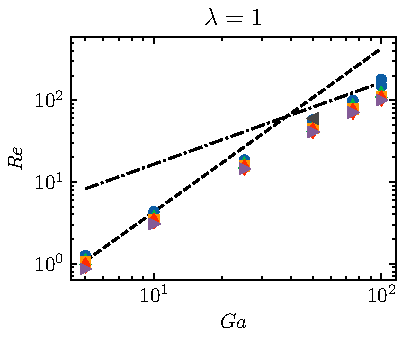
\includegraphics[height = 0.35\textwidth]{image/HOMOGENEOUS/fCA/Re_N_5_l_1.pdf}
    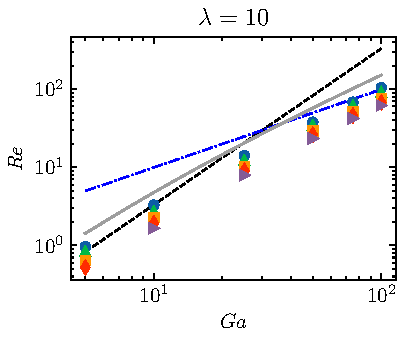
\includegraphics[height = 0.35\textwidth]{image/HOMOGENEOUS/fCA/Re_N_5_l_10.pdf}
    \caption{Reynolds number based on the slip velocity of the two phases as a function of $Ga$. ($\bullet$) $\phi = 1\%$, ($\blacktriangle$) $\phi = 5\%$, ($\blacksquare$) $\phi = 10\%$, ($\blacklozenge$) $\phi = 15\%$ and ($\blacktriangleright$) $\phi = 20\%$. (--) $Re \sim Ga ^2$, ($-\cdot-$) $Re \sim Ga ^1$.}
    \label{fig:Re_Ga}
\end{figure}

Within the Reynolds number range investigated in this study ($1 \lesssim Re \lesssim 100$), it is not possible to predefine the functional form of the drag force on the Reynolds number. This is illustrated in Figure \ref{fig:Re_Ga}. The figure reveals that the Reynolds number, based on the relative velocity, falls within the bounds of viscous scaling $Ga^1$ and inertial scaling $Ga^2$. It is noteworthy that increasing the volume fraction does not significantly modify the Reynolds number slope but simply shifts the points to higher $Ga$. Hence as in the previous subsection one may expect that separating the influence of the void fraction from the influence of the Reynolds number may be appropriate. This is a common approach, as seen in the widely applied Wen and Yu correlation \citep{wen1966}, employed for calculating forces in fluidized beds and sedimenting fluidized particles. Hence we assume that the mean force can be expressed as equation \ref{FCD}.


% la tendance est la meme quelque soit la frction volumique. Cela tends à nous indqiuer qu'un modele base sur un Cd isole qui va bien devrait fonctionner. En pratique il y a d'uatres modles (par exemple celui d'Ergun), amis dans le cas present il n'est pas adapté. Pour deux bonnes raison: deja il s'agit d'une superposition lineaire des deux 
%regimes lineaire et quadratique. PAr ailleurs il est fait pr des lits fixes

 





%\subsection{Steady drag force on an isolated spherical drop}
%First of all we want to investigate the dependency of the drift velocity with the volume fraction $\phi$. 
%It is known from several studies on the litterature, especially in \citep[chapter 8]{morel2015mathematical} and \citet[chapter 12]{ishii2010thermo} the the viscosity model for various system can be written generally, as,
%\begin{equation*}
%    \frac{\mu_m}{\mu_c}
%    = \left(
%        1 - \frac{\phi}{\phi_\text{max}}
%    \right)^{-2.5 \phi_\text{max}\mu_\text{eq}}
%\end{equation*}  
%with, $\mu_\text{eq} = \frac{\mu_d + 0.4 \mu_c}{\mu_d+\mu_c}$ and $\phi_\text{max}$ being the volume fraction corresponding to the \textit{maximum packing}. 
%\JL{la viscosite d'une suspension n'a rien a voir avec sa vitesse de chute meme si cela semble etre un argument donne dans la litterature... j'ai enleve tout cela pr l'instant}

%In this part, we briefly review the various formulas used to calculate the drag force on a spherical droplet embedded in a steady uniform flow.  Theoretical predictions for the force on a spherical droplet embedded in a steady uniform flow are limited to the limit of very small and very high Reynolds numbers. We define the drag coefficient, denoted as $C_D$ by the equation $F = \pi / 8 C_D \rho U_0^2 d^2$, where $F$ is the force on the drop, $U_0$ is the imposed velocity. The drag coefficient is a function of the Reynolds number $Re = \rho U_0 d /\mu $ and of is the viscosity ratio$\lambda = \mu _d /\mu _c$. % is the  as $F = C_D$ 
%In the Stokes regime ($Re=0$)the drag coeficient is given by the Hadamard-Ribczynski formula


%In this section, we briefly survey the diverse formulas applied to calculate the drag force acting on a spherical droplet within a steady, uniform flow. As corroborated in Appendix \ref{app:shape}, the droplet maintains an approximate spherical shape, a validity sustained across the entire spectrum of investigated parameters, even in the high inertial regime. Theoretical predictions for the force acting on a spherical droplet in a steady uniform flow are confined to scenarios of extremely low and exceptionally high Reynolds numbers.

%We define the drag coefficient, denoted as $C_D$, by the equation F=π8CDρU02d2F = \frac{\pi}{8} C_D \rho U_0^2 d^2F=8π​CD​ρU02​d2, where FFF signifies the force on the droplet, and U0U_0U0​ is the imposed velocity. This coefficient varies with the Reynolds number Re=ρU0dμRe = \frac{\rho U_0 d}{\mu}Re=μρU0​d​ and the viscosity ratio λ=μdμc\lambda = \frac{\mu_d}{\mu_c}λ=μc​μd​​. In the Stokes regime, the drag coefficient adheres to the Hadamard-Ribczynski formula.

%In the Stokes flow regime, the drag coefficient defined as $F = $

%drag force on a spherical drop embedded in a steady uniform flow is given by the Hadamard-Ribczynski formula
%\JL{il faut choisir ton echelle caractersitique de longueur. Soit $a$ le rayon soit le diametre des particules.}
%\begin{equation}
%F_0 = -\pi \mu d U \frac{2+3\lambda}{1+\lambda}
%\end{equation}

%\begin{equation}
%C_D = \frac{8}{Re} \left( \frac{2+3\lambda}{1+\lambda} \right)
%\end{equation}
%\ref{fig:U} shows the drift velocity $U$ divided by the stokes rising velocity of a spherical droplet $U_\text{stokes}$ defined in our notation as \citep{kim2013microhydrodynamics}, 
%Balancing the drag force obtained using the previous formula with the buoyancy force one obtained the settling velocity in the Stokes regime
%\begin{equation}
%    U_0
%    = (\rho_c - \rho_d)\frac{g d^2}{6\mu_c}\left(\frac{1+\lambda}{2 + 3\lambda}\right),
%\end{equation}
%or in dimensionless form 
%\begin{equation}
%    Re_0
%    = \frac{Ar^2}{6}\left(\frac{1+\lambda}{2 + 3\lambda}\right).
%\end{equation}
%where $Re_0 = \rho_c U_0 d/\mu_c$ is the Reynolds number based on the terminal velocity.
%In the opposite regime of very high Reynolds numbers ($Re\gg 1$), the flow outside the droplet can be considered as potential except in an infinitely thin boundary layer developing on the bubble surface. \citet{harper1968} have shown that the drag coefficient on a spherical drop is given by 

%\begin{equation}
%C_D = \frac{48}{Re}\left(1 + \frac{3\lambda}{2}\right).
%\label{eq:harper}
%\end{equation}
%Equation \ref{eq:harper} is the leading order expression in the expansion performed by \citet{harper1968} in the limit $Re\gg 1$. This equation tends toward Levich formula for the drag on a clean bubble in the limit $\lambda \ll 1$. A detailed investigation perfomed by \citet{dandy1989} have shown that the oroginal formulation by \citet{harper1968} became accurate for $Re\geq 200$. 

%Equation \ref{eq:harper} is the leading order term in the expansion carried out by \citet{harper1968} under the condition $Re\gg 1$. For $\lambda \ll 1$ this equation tends towards the Levich formula describing the drag on an uncontaminated bubble. A comprehensive investigation by \citet{dandy1989} revealed that the initial formulation proposed by \citet{harper1968} becomes accurate when $Re\geq 200$.

%\begin{equation}
%f_p (Re_s,\lambda,\phi) = C_D^0(Re_s,\lambda)g(\lambda,\phi)\frac{1}{8}\rho \pi d^2 |u-v|(u-v)
%\end{equation}
%where $C_D^0$ is the drag coefficient on an isolated drop and $g$ a function whose functional form is unknown \textit{a priori}.
Unfortunately in contrast to the Stokes regime there is no theoretical formula for the drag force on an isolated droplet for arbitrary Reynolds number. One may use potential flow theory (except in an infinitely thin boundary layer developing on the bubble surface) to predict the drag force on an isolated droplet in the limit  $Re\gg 1$ \citep{harper1968}, but numerical computations have shown that the theory is only accurate for $Re\geq 200$ \citep{dandy1989}.
%The above review show that in the intermediate Reynolds number regimes of the present study $ 1 \lesssim Re \lesssim 100$, there is no theoretical formulas. 
Hence in practice one have to rely on empirical relationship to predict the drag force on the drop. \citet{rivkind1970} proposed to write a drag force as a combination of the drag force on a solid spherical particle
(the limit ($\lambda \rightarrow \infty$) and the drag force on a spherical bubble ($\lambda \rightarrow 0$)

\begin{equation}
C_D^0(Re,\lambda) = \frac{C_{Ds}^0(Re)+\lambda C_{Db}^0(Re)}{1+\lambda}
\label{eq:CD0}
\end{equation}
where $C_{Ds}^0$ is the drag force on an isolated solid sphere and $C_{Db}^0$ the drag force on a shear-free bubble. Formula \ref{eq:CD0} constitutes a generalization of the Hadamard-Ribczynski formula in the intermediate Reynolds number regime. As suggested by \citet{magnaudet1997} we make use of the following correlation for the drag force on a solid particle and a bubble
\begin{align}
C_{Ds} ^0 &= \frac{24}{Re}(1+0.15Re^{0.687}) \\
%\end{equation}
%\begin{equation}
C_{Db} ^0 &= \frac{16}{Re}\left(1+\left[\frac{8}{Re}+\frac{1}{2}\left(1+3.315Re^{-1/2}\right)\right]^{-1}\right)
\end{align}
which where originally proposed by \citet{schiller1933} and \citet{mei1994} respectively. Formula \ref{eq:CD0} agrees with numerical results with an error of $5-7\%$ \citep{rivkind1970}.%Balancing the drag force obtained using the previous formula with the buoyancy force one obtained the settling velocity

%\begin{equation}
%C_D(Re)Re^2=\frac{4}{3}Ga ^2
%\label{}
%\end{equation}


%where higher order terms can be found in the original publication of \citet{harper1968}. 

%to leading order as $Re = \rho U_0 d /\mu$ 


%In practice the above formula are very limited randge of validity and empirical formulation have to be used for intermediate Reynolds numbers. Prendre la correlation de Rykind et Ryskin


%\begin{equation}
%nf_p = C_D(Re_s)\frac{3}{4}\frac{\rho _c |u_c-u_d|(u_c-u_d)}{D}\frac{\phi}{(1-\phi)^{n-3}}
%\end{equation}


%with $C_D^0$ given by "Jacques" Formula and  $h(\lambda,\phi)=\frac{1}{(1-\phi)^{n-3}}$
%We will now assume that the functional form of $f(\phi)$ is the same as in the Stokes flow regime and is thus indendent of the Reynolds number. This assumption, has no theoretical ground but \citet{di1994} has shown that $f$ is weakly dependent of the Reynolds number for solid particles. 
We will assume that the functional expression of $f$ remains the same with that observed in the Stokes flow regime, thereby assuming that it is independent of the Reynolds number. While this assumption has no theoretical ground, \citet{di1994} demonstrated that the dependency of $f$ on the Reynolds number for solid particles is small especially for low solid volume fraction.

%Hence for the sak

%This assumption, which have no theoretical ground has been shown to be rather accurate for spherical solid particles (). %Pour des bulles est ce le cas ? a on des résultats de vitesse de sedimentation pour different Ga ? a part Cartellier et Riviere. Je ne pense pas ils ne donnent pas la vitesse moyenne.



%\subsection{Hindered settling velocity}
%As an exemple for a suspenison of homogeneous solid spherical particle $\phi_\text{max} = 0.62$ and for deformable particles system it can be approximated to $\phi_\text{max} = 1$. 
%From this consideration we can deduce that the drift velocity $U$ is related to the volume fraction with, 
%\begin{equation*}
%    \frac{U(\phi)}{U_\text{stokes}} = \left\{\begin{tabular}{cc}
%        $(1-\phi)^{1.5}$   & bubbles in liquid \\
%        $(1-\phi)^{2.25}$   & drops in liquid \\
%        $(1-\phi)^{3}$   & drops in gas \\
%    \end{tabular}\right.
%\end{equation*}

 
%Additionally, \citet{bunner2003effect} propose a scaling of $\sim (1 - \phi^{1/3})$ for spherical bubbles.
%While \citet{ishii1979drag} proposed a $\sim (1 - \phi)^3$ for deformable bubbles. 




%In our case, i.e. quasi spherical droplets, we reach a $\sim (1 - \phi^{1/3})$ scaling for $\lambda = 10$ and approximately a $\sim (1 - \phi^{1/2})$ scalings for $\lambda = 1$ .
%\begin{figure}[h!]
%    \centering
%    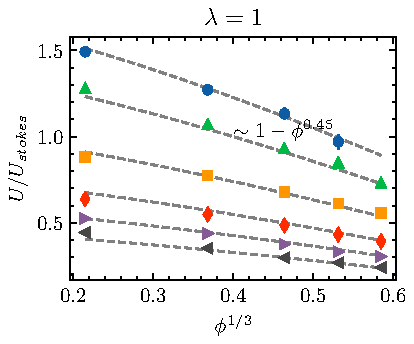
\includegraphics[height = 0.35\textwidth]{image/HOMOGENEOUS/fCA/UstokesGa_mu_r_1-0.pdf}
%    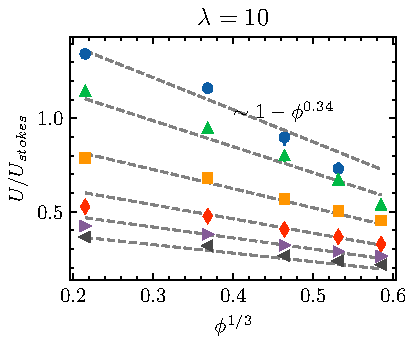
\includegraphics[height = 0.35\textwidth]{image/HOMOGENEOUS/fCA/UstokesGa_mu_r_0-1.pdf}
%    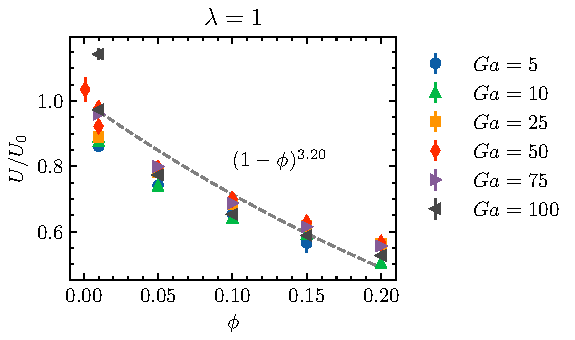
\includegraphics[height = 0.35\textwidth]{image/HOMOGENEOUS/fCA/Re_iso_N_5_l_1.pdf}
%    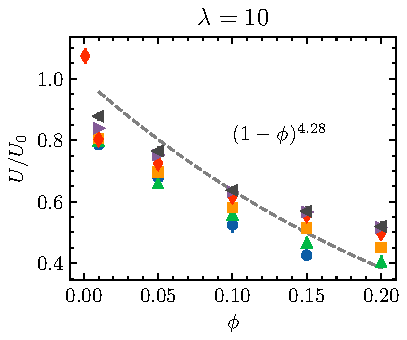
\includegraphics[height = 0.35\textwidth]{image/HOMOGENEOUS/fCA/Re_iso_N_5_l_10.pdf}
%    \caption{Rising velocity divided by the rising velocity of an equivalent spherical drop in Stokes regime.($\bullet$) $Ga = 5$, ($\blacktriangle$) $Ga = 10$, ($\blacksquare$) $Ga = 25$ , ($\blacklozenge$) $Ga = 50$, ($\blacktriangleright$) $Ga = 75$ and ($\blacktriangleleft$) $Ga = 100$ . 
%    The dashed lines are the empirical funtions (left)  
%    $U/U_\text{stokes} = 2.72(Ga^{-2.77} - Ga\;10^{-3}) (1 - \phi^{0.45})$
%    (right)  $U/U_\text{stokes} = 2.74(Ga^{-2.85} - Ga \;10^{-3}) (1 - \phi^{0.34})$ }
%    \label{fig:U}
%\end{figure}

%The case for which $\lambda = 1$ have a tendency to processes more deformation, as caracterised by their averaged aspect ratio $\chi$ slightly higher than those for which $\lambda = 10$. 
%The differences in the volume fraction dependency can be partially explain by this fact. 
%Indeed, a  $\sim (1 - \phi^{2/3})$ power law were observed for slightly deformable bubbly flow \cite{zhang2021direct}. 
%Thus it is not surprising that at low but finite deformation we found a scalings between $1/3$ and $2/3$. 

%A last interesting fact is that at low $Ga$ and $\phi$ we observe a rising velocity $U / U_\text{stokes} > 1$ meaning that the rising velocity is higher than in the stokes isolated case. 
%This phenomena has already been observe in \citet{loisy2017buoyancy}. 
%This fact was explained to be due to the cumulative effect of the wakes in orderred array of bubbles  which tends to increases their colective velocity. 
%Anyhow, since the the limit $Ga \rightarrow 0$ and $\phi \rightarrow 0$ we must recover $U/U_\text{stokes} = 1$ we can be sure that the $\phi$ scaling won't behaves like so.
%Therefore it is crucial to point out that these scalings are surely not valid in the limit  $Ga \rightarrow 0$ and $\phi \rightarrow 0$ .

%\subsection{Interphase drag force}




Now we present our results for the drag force term in terms of the Reynolds number. 
\begin{figure}[h!]
    \centering
    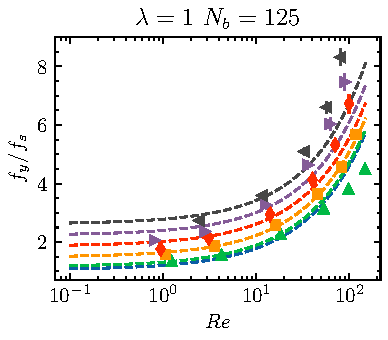
\includegraphics[height = 0.35\textwidth]{image/HOMOGENEOUS/fCA/Fstokes_N_5_l_1.pdf}
    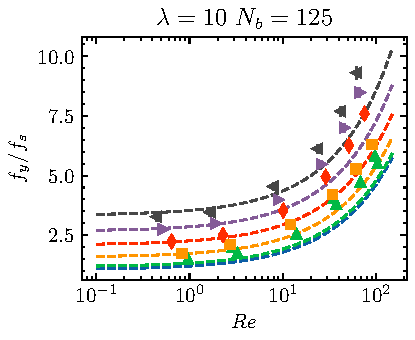
\includegraphics[height = 0.35\textwidth]{image/HOMOGENEOUS/fCA/Fstokes_N_5_l_10.pdf}
    \caption{
        (middle) Reynolds number based on the averaged rising velocity.
    (bottom) Ensemble averaged drag force divided by the stokes drag force on spherical droplet of equivalent size.
    The symbols correspond to different volume fraction ($\bullet$) $\phi = 1\%$, ($\blacktriangle$) $\phi = 5\%$, ($\blacksquare$) $\phi = 10\%$, ($\blacklozenge$) $\phi = 15\%$ and ($\blacktriangleright$) $\phi = 20\%$.
    (dashed lines) empirical formulas : extrapolation of  \citet{tenneti2011drag} for solid particles. }
    \label{fig:drag_force}
\end{figure}
\tb{As discussed in previous study that
for spherical bubbles, as the gas fraction increases and the in-
teractions become more important, the bubbles tend to align
themselves in horizontal pairs, whose average rising velocity
is lower than that of an isolated bubbl}

The interphase drag forces applied on the droplets is the buoyancy force $(\rho_d-\rho_c)v_\alpha \textbf{g}$.
The relevant quantity is therefore the dimensionless drag force, that is what is presented in the following \ref{fig:drag_force}. 


%In the stokes regime the drag force on a spherical droplet is, 
%\begin{equation*}
%    \textbf{F}_s
%    =\pi \mu_f d (\textbf{u}_p - \textbf{u}_c) \left(\frac{2+3\lambda}{1+\lambda}\right)
%\end{equation*}
%Let the dimensionless drag force be a function of $\lambda$ $Re$ and $\phi$, expressed such that, 
%\begin{equation}
%    \textbf{f}_p(Re,\phi,\lambda)
%    = 
%    f_1^*(Re)
%    f_2^*(\phi)
%    \textbf{f}_s(\lambda)
%\end{equation}
%where $f_{1,2}$ are coefficient which limit tends to $1$ at low $\phi$ and low $Re$. 
%To determine the $\phi$ dependency we base our study on the following analysis. 
%In \cite[chapter 4]{ashgriz2011handbook} they stipulate that the last droplets empirical fit was made in the study of \citet{rusche2000effect} where they performed empirical fits on experimental datas of emulsion. 
%Some of which concerned droplets' sedimentation, were they stipulate that, 
%\begin{align*}
%    f_1^*(\phi) 
%    &=1  + C_1 Re^{C_2}\\
%    f_2^*(\phi) 
%    &= e^{\phi K_1} + \phi K_2
%    \label{eq:drag_fit}
%\end{align*}
%Nevertheless, the coefficients for the droplets doesn't agree with our numerical calculation. 
%Instead we remark that the solid particles fit from \citet{rusche2000effect} well fits our results at $\lambda = 1$. 
%Therefore, we propose to keep the shape of teh fits and adjuste our coefficient. 

%\tb{Dans cette partie je ne sais pas trop quoi faire pour avoir un bon point de départ pour cree une formule empirique, je manque d'idée, notament pour ce qui est de la dépendence en $\lambda$ et pour l'explication physique des tendence observe. }
